

\documentclass[11pt]{article}

%\setlength\topmargin{-0.1in}
%\setlength\headheight{0in}
%\setlength\headsep{0in}
\setlength\textheight{8.5in}
\setlength\textwidth{6.5in}
\setlength\oddsidemargin{0in}
\setlength\evensidemargin{0in}
\usepackage{placeins}
\usepackage{indentfirst}
\usepackage{amsmath}
\usepackage{graphicx}
\usepackage{listings}
\usepackage{rotating}
\usepackage{subcaption} 
\usepackage{booktabs}
\usepackage{tikz}
\usepackage{siunitx}
\usepackage{fancyhdr}
\usepackage{pdfpages}
\usepackage{hyperref}
\usepackage{longtable}
%%Tables
\usepackage{booktabs}
\newcommand{\ra}[1]{\renewcommand{\arraystretch}{#1}}
%%Nomenclature
\usepackage{nomencl}
\makenomenclature
\newif\iffirstglossary\firstglossarytrue
%% This removes the main title:
\renewcommand{\nomname}{}
%% this modifies item separation:
\setlength{\nomitemsep}{8pt}
%% this part defines the groups:
%----------------------------------------------
\usepackage{etoolbox}
\renewcommand\nomgroup[1]{%
  \item[\Large\bfseries
  \ifstrequal{#1}{N}{Nomenclature}{%
  \ifstrequal{#1}{A}{List of Abbreviations}{}}%
]\vspace{10pt}} % this is to add vertical space between the groups.
%----------------------------------------------

\pagestyle{fancy}
\usetikzlibrary{shapes,arrows}
\graphicspath{{Figures/}}
\newcommand{\tabitem}{~~\llap{\textbullet}~~}

\newcommand*{\MyIndent}{\hspace*{0.5cm}}%inerts tab in tables

% Define FlowChart box styles
\tikzstyle{decision} = [diamond, draw, fill=blue!20, 
    text width=7em, text centered, inner sep=0pt]
\tikzstyle{block} = [rectangle, draw, fill=blue!20, 
    text width=7em, text centered, rounded corners, minimum height=2em]
\tikzstyle{line} = [draw, -latex']
\tikzstyle{cloud} = [draw, ellipse,fill=red!20, node distance=3cm,
    minimum height=2em]

 
\begin{document} 
\begin{titlepage}
	\newcommand{\HRule}{\rule{\linewidth}{0.5mm}}	
	\center
	\LARGE 
	University of Bath\\
 	Faculty of Engineering \& Design\\[1cm]	
	%\textbf{\Large ME30313 Group Business & Design}\\
	\large
	Word count: 2529\\[0.5cm]
	{\large\today}\\[1cm]	
	\HRule\\[0.4cm]	
	{\huge\bfseries Technical Integrators Report}\\[0.4cm] 	
	\HRule\\[1cm]	
	\begin{minipage}{0.4\textwidth}
		\begin{flushleft}
			\large
			\textit{Supervisor}\\
			J. \textsc{Jupp}
		\end{flushleft}
	\end{minipage}
	~
	\begin{minipage}{0.4\textwidth}
		\begin{flushright}
			\large
			\textit{Assessor}\\
			J. \textsc{Jupp} 
		\end{flushright}
	\end{minipage}\\[1.4cm]
	\large
	\textit{Author}\\
	Xavier \textsc{Forde}\\
	\vfill
	
\includegraphics[width=0.4\textwidth]{UOB_Logo.png}\\
	\vfill 
\end{titlepage}

\section*{Executive Summary}
The UOB100 is a 100 seater regional jet designed for 1000 nautical mile missions or three 300nm missions without refueling. The configuration chosen is a high wing turboprop similar to competitor aircraft: the ATR72 and Bombardier Dash 8 Q400. The project also comprised an 80 seater family member tailored to to the 300nm hop missions.

\newpage

\tableofcontents
\listoffigures
\listoftables

\nomenclature[A]{AR}{Aspect Ratio}
\nomenclature[A]{CFRP}{Carbon Fibre Reinforced Polymer}
\nomenclature[A]{CG}{Centre of Gravit}
\nomenclature[A]{DOC}{Direct Operating Cost}
\nomenclature[A]{FOD}{Foreign Object Damage}
\nomenclature[A]{G.D.}{General Dynamics}
\nomenclature[A]{HTP}{Horizontal Tailplane}
\nomenclature[A]{MAC}{Aerodynamic Mean Chord}
\nomenclature[A]{MLG}{Main Landing Gear}
\nomenclature[A]{MTOW}{Maximum Take-Off Weight}
\nomenclature[A]{NLG}{Nose Landing Gear}
\nomenclature[A]{VTP}{Vertical Taiplane}
\nomenclature[A]{SUGAR}{Subsonic Ultra Green Aircraft Research}


\printnomenclature

\clearpage

\section{Introduction}

A team of students from the University of Bath have been tasked with designing a 100-seat and an 80-seat regional aircraft family to serve both 1000nm and 3x300nm missions. The aircraft were to conform to a predetermined design specification\cite{SPEC} which defined standard dimensions and performance characteristics. The aircraft will be in direct competition with the ATR 72-600 and the Bombardier Dash 8 Q400, with the aim of reducing DOC (direct operating costs) 15\% compared to these aircraft. \\
The Technical Integrator's role was to develop and control the overall configuration in conjunction with the technical specialists. The primary design driver for any aircraft program is conformity to safety regulations, EASA's CS-25 \cite{CS25} in this case. Aside from safety, the target DOC reduction was the driver behind major design decisions. The aircraft configuration was developed to best meet this aim was a high wing turboprop with a T-tail aircraft configuration.\\
The aircraft family name is the A3UX and the family members are the A3U10 100 seater and the A3U8 80 seater.
\\
Another role of the Technical Integrator was estimation and control of aircraft weights and and balance. Accurate weight estimation is a priority in any civilian transport aircraft program, incorrect weight estimation can lead to over optimistic DOC estimates for light estimates and necessary structural weight being added to support heavy estimates. A weight breakdown was needed by every member of the team to analyze and size components such as engines and lifting surfaces, which in turn were needed for the weight estimates. As the Technical Integrator was responsible for the layout of these components it is sensible that this role should also control the weights and their positions.\\It is also essential that the aircraft is balanced correctly and is always kept within CG limits so that the the pilot has sufficient control over the aircraft for safe flight. Therefore weight balance diagrams were made to ensure this was the case for all load cases.
\\
As technical specialists work on detailed design the perspective of the overall configuration can sometimes be lost. The Technical Integrator role was therefore important in ensuring each aircraft component was designed to suit the aircraft configuration as a whole and work with specialist roles when integration issues arose.\\

\section{Aim}
The primary aim of this report is to present and justify the configuration of the aircraft primarily in terms of DOC impact. In addition the weight of the aircraft is to be assessed and CG postions for all flight cases found, with any loading restrictions defined.

\section{Scope}

The primary focus for the report is the A3U10 aircraft as this heavier aircraft will be the limiting design case for the majority of components. Therefore repeating the A3U10 seat calculations in the same level of detail for the A3U8 is beyond the scope of this report and so there is greater uncertainty in the parameters stated for the A3U8. The overall design and configuration of the A3U8 shall be assessed however to show commonality between designs.

\section{Main Parameters and Data Control}

The platform for maintaining the main parameters of the aircraft was not changed from phase 2. This was a cloud based spreadsheet that could be accessed by any of the team members, but with read-only access. Changes to this spreadsheet had to be requested and approved by the Technical Integrator and a log was kept of the approved changes along with the reason for change which is available in Appendix XXXX. A second copy of this spreadsheet was kept for intermediate calculations during iterative design processes. For example the Technical Integrator approved an increase in fuselage diameter, this changed the weight and drag polar, which in turn required a new engine scaling. Some iterations were needed to converge on the new weights and engine scales and logging all of these changes would not be practical. Therefore only the final iterations were added to the primary database. \\
In the primary database every parameter was assigned a responsible team member dependent on how important that parameter was to the team member's work. These parameters could not be changed without prior approval from the responsible member as well as the Technical Integrator. The team members responsible for each parameter can be found in Appendix XXX\\
The final revision of the parameter database is shown in Table \ref{table:PDB}.

\pagebreak

\subsection{End of Phase 3 Aircraft Parameters}


\begin{center} %PARAMETER DATABASE
\begin{longtable}{lll}
\caption[Main Aircraft Paramaters]{Main Aircraft Paramaters.} \label{table:PDB} \\

\hline \multicolumn{1}{l}{$Parameter$} & \multicolumn{1}{l}{$Value$} & \multicolumn{1}{l}{$Unit$} \\ \hline 
\endfirsthead

\multicolumn{3}{c}%
{{\tablename\ \thetable{} -- continued from previous page}} \\
\hline \multicolumn{1}{l}{$Parameter$} &
\multicolumn{1}{l}{$Value$} &
\multicolumn{1}{l}{$Unit$} \\ \hline 
\endhead

\hline \multicolumn{3}{r}{{Continued on next page}} \\ 
\endfoot


\endlastfoot

\midrule
\textbf{Weights}\\
Maximum Take-Off Weight&31,675&kg\\
Operators Weight Empty&18,790&kg\\
Maximum Landing Weight&30,790&kg\\
Maximum Zero Fuel Weight&28,290&kg\\
Mission Block Fuel (1000nm)&2,653&kg\\
Hold \& Reserves Fuel&692&kg\\
Maximum Fuel Capacity&4027&kg\\
\midrule
\textbf{Performance}\\
Cruise Mach Number & 0.5 &\\
VC & 197 &KEAS\\
Initial Cruise Altitude & 26,000&ft \\
L/D (Start of Cruise) & 17.5 & -\\
Take-Off Field Length & 852 &m\\
Landing Field Length & 757 &m\\
Approach Speed & 112 & kts\\
\midrule
\textbf{Fuselage}\\
Fuselage Length &29.34 & m\\
Fuselage Diameter &3.397 &m\\
\midrule
\textbf{Wing}\\
Area & 83 & m$^{2}$\\
Span & 32.85 & m\\
Aspect Ratio & 13 &\\
Tip Thickness (t/c) & 0.17 / 0.13& \\
Taper Ratio & 0.34 & \\
Root Chord & 3.532 &m\\
Tip Chord & 1.20 &m\\
Sweep 1/4 Chord & 2.3 & degrees\\
High Lift System (Flap Type) &Single Slotted Fowler&-\\
High Lift System (Slats) & None&-\\
C$_{L,MAX,LAND}$ & 3.03&\\
Distance From Nose to Root LE & 11.91 & m \\
Distance From Nose to MAC LE & 12.36 &m\\
Dihedral & 4 & degrees \\
\midrule
\textbf{Horizontal Tailplane}\\
Area & 19.5 &m$^{2}$\\
Span & 32.85 & m\\
Aspect Ratio & 6 &\\
1/4 MAC Wing to 1/4 MAC HTP & 15.29 \\
\midrule
\textbf{Vertical Tailplane}\\
Area & 17.4 &m$^{2}$\\
Span & 5.28 & m\\
Aspect Ratio & 1.6 &\\
1/4 MAC Wing to 1/4 MAC VTP & 13.69&m \\
\midrule
\textbf{Engine}\\
Number of Engines & 2 & - \\
Wing or Fuselage Mounted & Wing &-\\
Engine Scale (of TF80) & .807 & - \\
Sea Level Static Thrust (per Eng.) & 47,923 &kN\\
Thrust at Initial Cruise Alt. (per Eng.) & 8,956 &kN\\
\midrule
\textbf{Landing Gear}\\
MLG Tyre Size & & \\
Main Landing Gear Geometry for ACN &Twin Wheel Nose \& Main &\\
Height of Fuselage above Ground &2.15 &m \\
Height of Cargo Floor Above Ground &1.2 &m\\
\midrule
\textbf{Financial} \\
Aircraft NRC& 1.48 &Million \$ \\
Aircraft RC& 14.7&Million \$ \\
Fleet Initial Investment &1,300 &Million \$ \\
Operating/Support Costs & &Million \$ \\
Disposal Costs & &Million \$ \\

\bottomrule
\end{longtable}
\end{center}



\section{Configuration}

Although the parameter database controlled much of the data needed by specialists for their analysis the General Arrangement drawings shown in Figures \ref{fig:ga100} and \ref{fig:ga80}, with higher quality versions appended, controlled the layout and geometric shape of the aircraft, as well as giving perspective to the parameter values in the database. The General Arrangement drawings were also important to weight calculations and empennage sizing, giving distances between aerodynamic centres of lifting and control surfaces. \\
Examination of the General arrangement drawings will show that both aircraft have a common wing, nose, tail, empennage and landing gear. The difference geometric difference between the two aircraft is the shortened section of parallel fuselage for the 80 seater variant. The 80 seater will also have smaller landing gear wheels but this has not been assessed and will not cause integration issues. The use of a common wing will cause a sub 80 seater is sub-optimal in terms of weight and drag, increasing fuel burn, but this will be off-set by the greatly reduced recurring and non-recurring production costs.

\FloatBarrier
\begin{figure}[!h]

\centering
\includegraphics[angle=90,origin=c, width=0.9\textwidth]{100_ga.png}
\caption{A3U10 General Arrangement Drawing}
\label{fig:ga100}
%\end{turn}
\end{figure}


\begin{figure}[!h]
\centering
\includegraphics[angle=90,origin=c, width=0.9\textwidth]{80_ga.png}
\caption{A3U8 General Arrangement Drawing}
\label{fig:ga80}
%\end{turn}
\end{figure}
\FloatBarrier

\subsection{Configuration Selection}

The design process began with a brainstorm of possible configurations. This lead to the development of a phugh matrix which can be seen in Figure \ref{fig:pugh}. Using the pugh matrix some conventional as well as some novel concepts were generated. The concepts were compared to the current competition and from this two were selected for a final evaluation, one conventional and one more novel. The first concept, shown in Figure \ref{fig:concept1} was a high wing turboprop, similar to the ATR 72 and Bombardier Dash 8. The second concept, shown in Figure \ref{fig:concept2}, was a braced wing turbofan similar to the NASA - Boeing ‘SUGAR’ \cite{SUGAR}.


\begin{figure}[!h]
\centering
\includegraphics[width=0.9\textwidth]{pugh.png}
\caption{Pugh Matrix of Configuration Options }
\label{fig:pugh}
\end{figure}

\begin{figure}[!h]
\centering
\includegraphics[width=0.9\textwidth]{concept1.png}
\caption{High Wing Turbofan }
\label{fig:concept1}
\end{figure}

\begin{figure}[!h]
\centering
\includegraphics[width=0.9\textwidth]{concept2.png}
\caption{Braced Wing Concept}
\label{fig:concept2}
\end{figure}


\FloatBarrier

The braced wing was an interesting concept. It would allow for a very high aspect wing, reducing wing drag, without the increased weight usually associated with high AR wings due to the bracing. For a 1000nm mission the increased drag in cruise due to the bracing wing would outweight the wing drag saving, which is why braced wings are more common small general aviation aircraft. Concept 1 was chosen to advance into the next design stage. The use of turboprop propulsion was the primary driver behind this choice. This is beacuse over the short missions defing in the specification the turboprop engine was qulatively judged to offer lower fuel burn than a turbofan. The difference was thought to outweigh the aerodynamic or weight advantages of the other concepts. Furthermore the concentional design would reduce development time and costs which was a concern due to the 2025 entry into service requirement and the contribution to DOC respectively \cite{spec}. The concept was a starting point for more detailed analysis to prove the DOC reduction and optimisation of design. 

\subsection{Engines}

The mission distances defined in the specification are 1000nmi for the A3U10 and three 300nm hops for the A3U8. For flexibility the aircraft should be able to complete both missions however. The. The  2 reduce maintenance over 4 Turbofan engines were chosen as they reduce fuel burn over the mission distances. The decision was somewhat qualitative as it is known competitor aircraft the ATR-72 and Bombardier Dash-8  both use turboprops for this reason. The assessment was  

\subsection{Engine Integration}

The engines are mounted below the wing with the nacelles blended into the leading edge of the wing to create maintain airflow over the upper surface of wing, thereby increasing $C_{L_{MAX}}$.\\

The engines must be high to avoid ingestion of foreign object as discussed in section 5.5. XXXXX%CHECK THIS IS UP TO DATE


\subsection{Fuselage}

A 5-abreast fuselage was chosen in the second phase of the design and this has not changed. The CS 25.807 \cite{CS25} requirement of a maximum 60 feet distance between emergency exit doors was one of the drivers for this decision. To meet this requirement a 4-abreast cabin would require two Type III mid cabin in the 100 seater configuration. Furthemore the longer fuselage required for 4-abreast seating arrangement will reduce the maximum allowable rotation angle for take-off and landing. The rotation angle at take-off for the A3U10 is \ang{9.5}\cite{josh} and the maximum allowable is \ang{11.0} as shown on the the General Arrangement drawing. This gives a small safety margin of \ang{1.5} which would dissapear with the 4m extra fuselage length needed for a 4-abreast arrangement. 

\subsection{Fuselage Geometry}

The fusealge can contribute between 25 and 50 percent of total drag \cite{R3} and typically 7 to 12 percent of MTOW \cite{jenk}. Therefore it is important that is of the correct size and shape. The fuselage geometry for the A3U8-Mallard 100 seat variant can be seen in Figure \ref{fig:fgeo}.The fuselage has a parallel section for the cabin with a circular cross-section. This means the 80 seater variant can be easily made by removing parralel fuselage sections from the 100 seater design, and similarly a stretch variant could be made by adding parralel fuselage sections \cite{GAPP}. Furthermore the circular section is optimal for pressurisation, thereby reducing fuselage weight, and is easy to manufacture \cite{R2}.  The nose and tailcone section were sized and shaped to minimize drag. Values for tailcone fineness, nose taper length, fuselage fineness, rear pressure bulkhead position and tailcone upsweep angle are suggested by Roskam \cite{R2} and Schmitt \cite{SCHMITT} and a shown in Table \ref{table:fgeo}.


\begin{figure}[h!]
\centering
\includegraphics[width=0.9\textwidth]{fuse_geo.PNG}
\caption{Definition of Fuselage Geometry and 100 Seater Values}
\label{fig:fgeo}
\end{figure}


\begin{table}[!h]
\centering
\ra{1.3}
\begin{tabular}{@{}rrrrrr@{}}\toprule
& \multicolumn{5}{c}{$Ratio$}\\
\cmidrule{2-6}
&$L_{Bug} / D_f$&$L_f / D_f $&$L_{KabE} / D_f$&$L_{fc} / D_f$&$\theta_{fc} (deg)$\\ \midrule
$Roskam$& - &5.6-10& - &2-4&15-19 \\
$Schmit$&$\sim$1.7&-&$\sim$1.9 &3.5&- \\ \midrule
$A3UX (100)$&1.4&8.6&2.1&3.3&14.6 \\
$A3UX (80)$&1.4&7.7&2.1&3.3&14.6 \\
\bottomrule
\end{tabular}
\caption{Comparison of Reccommended Geometry}
\label{table:fgeo}
\end{table}


The values presented by Roskam are specifically for regional transports whereas Schmitt values are for transporters in general. The ratios for the A3UX 100 seat and 80 seat variants are shown Table \ref{table:fgeo} for comparison. The nose length to fuselage diameter ratio, $L_{Bug} / D_f$, is less than the value recommended by Schmitt. Increasing the nose section taper further would require reducing the height of the cabin where passengers board which is undesirable. The ratio is more applicable to transonic aircraft which would experience shock waves, and resulting noise and compressibility drag, with a blunt nose. The A3UX design cruise speed is 0.54 MACH XXX, and so shock waves forming at the nose is not an issue, however the ratio is close to the recommended value in order to reduce noise at the front of the aircraft. \\
The fuselage fineness ratio, $ L_f / D_f$, is within the typical range presented by Roskam. The minimum tube drag is occurs at a fineness ratio of approximately 6, however the reduction in empennage weight associated with a longer fuselage means the ideal fineness ratio is approximately 8. As the fineness ratios for the 80 and 100 seater variants fall either side of the ideal value the 5-a-breast layout is further justified. \\
The fuselage cone fineness ratio, $L_{fc} / D_f$, and upsweep angle, $\theta_{fc}$, are important in reducing upsweep drag. The value for the tailcone fineness ratio is in the range for regional aircraft and close to the value suggested by Schmitt. This is important as a short tail section will increase drag and a long tail section will increase weight, and therefore also increase drag. The upsweep angle is important in keeping attached flow over the tailcone and, when rounded to two significant figures, fits the range for regional aircraft presented by Roskam. The upsweep drag has been evaluated by the aerodynamic specialist and the aircraft will cruise at a \ang{1.6} nose up incidence to minimise it \cite{kit}. 



\subsection{Wing}

The A3UX has a high wing which is suitable for this application for several reasons. The high wing is necessary to give sufficient ground clearance for the propellers. The target market for the A3UX is developing countries with challenging terrain. Therefore it is essential that the aircraft is reliable on rough runways. Keeping the engines high reduces the chance of foreign object damage (FOD). The high wing also allows larger propellers to be installed, reducing the revolutions per minute (RPM) required for a given thrust, and thereby engine noise. \\
A further advantage of the high wing is the clean upper surface of the aerofoil, this provides more lift and therefore shorter runways are needed for take-off. The take-off performance is further improved as the flaps can extend partially into the fuselage diameter, increasing wing effective area \cite{kit}. As achieving the take-off field length of 1400m defined in the specification \cite{SPEC} was critical in sizing the engines \cite{josh} the increased lift from the high wing reduced engine weight.\\
One of the drawbacks of the high wing is difficulty of maintenance. The Fowler flaps and ailerons are to high to be inspected from the ground, the same applies for the engine. Furthermore the high wing means landing gear mounted into the wing or even engine nacelle would have to be significantly longer, and therefore heavier, than landing gear integrated into a low wing. This weight penalty has is not as applicable to the A3UX family as the landing gear is fuselage mounted, however this requires a blister fairing which causes additional drag.


\subsection{Empennage}

As can be seen in Figures \ref{fig:ga100} and \ref{fig:ga80} the A3UX family feature a common T-tail empennage. The main driver behind this decision was keeping the HTP (horizontal tailplane) clear of propeller slipstream, meaning it will not be affected by changes in engine thrust. In the T-tail design the HTP acts like an endplate for the VTP (vertical tailplane), reducing drag. The VTP for the A3UX family also has a \ang{25} quarter chord sweep as shown in Figures \ref{fig:ga100} and \ref{fig:ga100} which increases the lever arm of the HTP. This allows a smaller, and lighter, HTP but the weight advantage is likely to be outweighed by the additional weight required to stiffen the VTP to support this weight. This VTP weight increase was calculated to be 16\% \cite{tbeek}. A slight \\ 
A common problem with T-tail configurations is deep stall, however the high wing means horizontal tailplane will be below the wake of the stalled wing so deep stall is not expected to be a concern. A slight anhedral of ang{0.5} was applied to the HTP which has been shown to produce better flutter resistance and therefore reduce weight \cite{R3}. The HTP aerofoil was also changed from NACA0009 to NACA0012, as recommended in the phase 2 feedback, \\ CAN TALK ABOUT THE RUDDER AND elevator. ALSO THE HTP THICKNESS WAS INCREASED TO REDUCE WEIGHT.

\subsection{Empennage Integration}

The main concern with empennage integration was keeping the front spar of the VTP aft of the rear pressure bulkhead \cite{GAPP}. There were no major changes to the empennage since the second phase, only a small decrease in areas which aided in the rear spar location.	 The spar, at 15\% chord, is indeed still clear of the rear pressure bulkhead as Figure \ref{fig:vtpspar} demonstrates.

\FloatBarrier
\begin{figure}[h!]
\centering
\includegraphics[width=0.9\textwidth]{vtp_spar.PNG}
\caption{Rear Pressure Bulkhead and VTP Front Spar Locations}
\label{fig:vtpspar}
\end{figure}
\FloatBarrier

\subsection{Landing Gear}

As can be seen in the general arrangement drawings a tricycle arrangement, with fuselage mounted landing gears, was chosen for the A3UX family. The arrangement is similar to the BAe-146 and ATR-72 large regional aircraft. This was choice was driven by the high wing configuration which would make wing or engine nacelle mounted MLG (main landing gear) longer and heavier than the fuselage mounted design. The nose landing gear has not changed significantly from the previous phase. It is mounted 2.7m from the nose whilst the MLG is located at 52.5\% MAC (mean aerodynamic chord). As required by CS-25.729 there must be two means of deploying the nose landing gear \cite{CS25}. As a result the nose gear retracts forward into the fuselage so in case of system failure gravity and aerodynamic drag will deploy the landing gear. To save manufacturing and design costs the landing gear shall be common between the two aircraft so has been sized for the 100 seater A3U10.  

\subsection{Landing Gear Integration}

During the second phase of design a large blister fairing was required to store the MLG as shown in Figure \ref{fig:mhedi}. The drag penalty incurred by such a fairing would negate the weight saved by fuselage mounting the landing gears. Therefore work was done in the third design phase to reduce the size of the landing gear and fairings. This effort was helped by a significant drop in MLW (maximum landing weight) from 3580kg to 30790kg and as a result the landing gear was almost completely resized. The team did not have a landing gear specialist member in phase three so the sizing was completed using some analysis and comparison with similar aircraft. A 36in MLG tire diameter was chosen after comparison with the ATR 72-600 \cite{jane}, Bombardier Dash-8  Q400 \cite{q400} and BAe 146 300 series \cite{bae146} as shown in Table \ref{table:MLG}. \\
 The track was reduced from the phase 2 value of 6206mm to 4766mm. It is suggested that for good ground stability of the aircraft it should have a maximum lateral tip angle of \ang{55} at forward CG limit \cite{GAPP} as shown in Figure \ref{fig:geartip}. Using the detailed weight and position breakdown of the aircraft presented later in the report the location of the forward CG was found to be 12\% MAC at a height 3100mm above the ground. The MAC is 2745mm and the CG position is 40.5\%MAC ahead of the MLG equating to 1112mm. A CAD (computer aided design) model was made of the CG position and wheel positions as shown in Figure \ref{fig:xfgeartip}. The lateral tip angle was then shown to be \ang{56}. Despite this being slightly higher than the recommended \ang{55} it is deemed acceptable as the track is wider than the BAe146 which is a larger aircraft and there is a reasonable amount of uncertainty in the height of the CG position.\\
The end result of these changes is a more compact retraction mechanism and much smaller blister fairing for the third phase as shown in Figure \ref{fig:xgears}. Without the reduction in drag associated with the smaller blister fairing it is highly unlikely the 15\% DOC reduction target could have been met.


\FloatBarrier
\begin{table}[!h]
\centering %COMPARISON OF TIRE SIZES
\ra{1.3}
\begin{tabular}{@{}llll@{}}\toprule
$Aircraft$ & $MLW$ & $Tire \ Size$ & $Track$ \\
\midrule
ATR 72-600 & 22,350kg & 34in  & 4.1m\\
Dash-8 Q400 & 27,442kg & 34in & 8.8m \\ 
BAe 146 300Series & 37,648kg & 39in & 4.72m \\
\midrule
 A3U10 & 30,790(kg) &  36(in)& 4.76(m)\\
\bottomrule
\end{tabular}
\caption{Comparison of Main Landing Gear Configuration}
\label{table:MLG}
\end{table}

\FloatBarrier
\begin{figure}[h!] %Mhedi Gears
\centering
\begin{minipage}{.5\textwidth}
	\centering
	\includegraphics[width=0.9\linewidth]{landgeargeo.PNG}
	\captionof{figure}{Later Tip Angle Geometry \cite{GAPP}.}
	\label{fig:geartip}
\end{minipage}%
\begin{minipage}{.5\textwidth}
	\centering
	\includegraphics[width=0.9\linewidth]{land_gear_cad.png}
	\captionof{figure}{Demonstration of Maximum Lateral Tip Angle: \ang{56.27}.}
	\label{fig:xfgeartip}
\end{minipage}
\end{figure}


\begin{figure}[h!] %Mhedi Gears v xavi gears
\centering
\begin{minipage}{.5\textwidth}
	\includegraphics[width=1\linewidth]{mhedi.PNG}
	\captionof{figure}{Phase 2 Landing Gear Intergration}
	\label{fig:mhedi}
\end{minipage}%
\begin{minipage}{.5\textwidth}
	\centering
	\includegraphics[width=01\linewidth]{xfgears.PNG}
	\captionof{figure}{Improved Landing Gear Intergration For Phase 3}
	\label{fig:xgears}
\end{minipage}
\end{figure}

\subsection{Commonality between designs}

\section{Weights and Balance} 

\subsection{Weight Estimation}

The estimate for aircraft weight is crucial in sizing the lifting surfaces, structural and propulsive components as well determining fuel burn - a direct contributer to DOC. Therefore it is crucial that weight estimations are accurate and reliable, in order to achieve this several methods were used to estimate the weight of aircraft components. The results for the four methods used are shown in Table \ref{table:w_est}. There is some significant variation in component weights between methods, specificaly the Jenkinson \cite{jenk} method tended to be higher than that of the Torenbeek \cite{tbeek} and G.D. (General Dynamics) \cite{R5} methods. As Jenkinson formulas tend to be a strong function of MTOW and so are intended as a preliminary estimate, these values have been not been used. The Guide method \cite{guide} is a combination of several other methods, meaning a greater chance of double counting weights, and so has also not been used. The Torenbeek and G.D. methods require a significantly greater number of parameter inputs and therefore are likely to be more represetative of the aircraft. Therefore a combination of these two methods has been used depending on which estimation was most suited to the A3U10 configuration. The A3U10 weights appear in the final column and have been highlighted bold to show which method was used.\\
A further motivation for using the Torenbeek and G.D. method was the greater break down of weights. This provided better estimates for CG positinos than possible for the Jenkinson method which bundled fixed equipment into one weight. 


\begin{table}[!h]
\centering
\ra{1.3}
\begin{tabular}{@{}rrrrrr@{}}\toprule
& \multicolumn{5}{c}{$Weight (kg)$}\\
\cmidrule{2-6}
&$G.D. \ Method$&$Torenbeek$&$UoB \ Guide$&$Jenkinson$& \textit{\textbf{A3U10}}\\ \midrule
\textbf{Structures}\\
Wing Group& 3841   & \textbf{4045}& 5069 &3801&\textbf{4045}\\
Fuselage Group&3619&\textbf{4170}& 5088 &5032&\textbf{4170}\\
\MyIndent (Horizontal \ Tailplane)&(226)& (245)& - &(488)&(226)\\
\MyIndent (Vertical \ Tailplane)&(265)&(251)& - &(487)&(265)\\
Empennage&\textbf{491}& 497 & 869 & 974 &\textbf{491}\\
Land. Gear Group&\textbf{1092}&1003&1292&1377&\textbf{1092}\\
\cmidrule{2-6}
Structure \ Total&9043&9715&12318&11185&\textbf{9798}\\
\cmidrule{2-6}
$\textbf{Fixed Equipment}$\\
Fuel Systems&\textbf{129}&276&234&-&\textbf{129}\\
Flight Controls \& Hydraulics&602&\textbf{526}&559&479&\textbf{526}\\
Avionics&404&\textbf{282}&376&-&\textbf{282}\\
Electrical Systems&\textbf{502}&444&922&-&\textbf{502}\\
Air Cond. Systems&\textbf{939}&637&1557&-&\textbf{939}\\
Furnishings&\textbf{267}& - &1108&-&\textbf{267}\\
\cmidrule{2-6}
Fixed \ Equipment \ Total&2843&2432&4756&2580&2645 \\
\cmidrule{1-6}
Structure\ + Fixed \ Eq. Total&11886&12147&17074&13765&\textbf{12443}\\

\bottomrule
\end{tabular}
\caption{Weight Estimation of A3U10 Using Several Methods}
\label{table:w_est}
\end{table}

\FloatBarrier



\subsubsection{Wing Weight Estimation}

The Torenbeek method was selected for the wing weight estimation because the G.D. method is only valid for aspect ratios up to 12 and the A3U10 has an aspect ratio of 13. Equation \ref{eq:wing} is the Torenbeek formula for wing weight estimation.\\
The definition of the parameters and their values is shown in Table \ref{table:wing}. Both the Torenbeek and G.D. formulas are for use imperial units but the metric equivelants have been included in the table for ease of consistency.


\begin{equation} \label{eq:wing} %%Wing Equation
\begin{split} 
W_{wing} = 0.001*MZFW*(b /& cos(\Lambda_{\frac{1}{2}}))^{.75}*[ 1 + (6.3*cos(\Lambda_{\frac{1}{2}})/b]^{0.5}*N_{ult}^{0.55}* \\
 & *(bS / t_{r}*MZFW*cos(\Lambda_{\frac{1}{2}})^{0.30}
\end{split}
\end{equation}

\begin{table}\centering    %Wing Table
\ra{1.3}
\begin{tabular}{@{}llll@{}}\toprule
$Parameter$ & $Definition$ & $Metric \ Value$ & $Imperial \ Value$ \\
\midrule
$MZFW$& Maximum Zero Fuel Weight & 28,290kg & 62,369lb \\
$b$ & Wing Span & 32.85m & 107.8ft \\ 
$\Lambda_{\frac{1}{2}}$ & Hald Chord Angle of Sweep & \ang{0} & \ang{0} \\
$t_{r}$& Maximum Thickness of Wing Root Chord & 0.6m & 1.97ft \\
$N_{ult}$& Ultimate Load Factor & 3.5 & 3.5 \\
\midrule
$W_{wing}$ & Wing Group Weight & 4,045kg & 8,918 lb \\
\bottomrule
\end{tabular}
\caption{Parameters For Wing Weight Group Estimation}
\label{table:wing}
\end{table}
\FloatBarrier

\subsubsection{Fuselage Weight Estimation}

The Torenbeek method was again used for the fuselage weight estimation, the formula for which is given by equation \ref{eq:fuse}. This is because it contained a factor for fuselage mounted landing gear such as that on the A3U10. Furthermore it was felt that using fuselage gross shell area was more accurate than relying on fuselage length and diameter which was the case for the other methods. The pressurisation factor $K_f$ was reduced from 1.08 to 1.06 as the A3U10 will cruise at 27,000ft XXX which is much lower than typical civilian transport planes which cruise around 40,000ft and so will not need the same level of strengthening material. The parameter definitions are given in Table \ref{table:fuse}.

\begin{equation} \label{eq:fuse} %Fuselage Equation
\begin{split} 
W_{fuse}& = 0.021*K_{f}*V_{D} * \big( L_{h} / (w_{f} + h_{f}) \big) ^{0.5}*S_{fgs}^{1.2} \\
&where \ the \ constant \ K_{f} \ takes \ the \ following \ values:  \\
&K_{f} = 1.08 \ for \  a \ pressurised \ fuselage \\
&\ \ \ \ = 1.07 \ for \ a \ main \ gear \ attached \ to \ the \ fuselage
\end{split}
\end{equation}


\begin{table}[!h]
\centering %Fuselage Table
\ra{1.3}
\begin{tabular}{@{}llll@{}}\toprule
$Parameter$ & $Definition$ & $Metric \ Value$ & $Imperial \ Value$ \\
\midrule
$K_f$& Constant & 1.14 & 1.14 \\
$V_D$ & Design Dive Speed & \multicolumn{2}{c}{245 KEAS} \\ 
$L_{h}$ & Distance from 25 \% Wing MAC to 25\% HTP MAC & 15.18m & 49.8ft \\
$w_{f}$ & Fuselage Width & 3.397m & 11.1ft \\
$h_{f}$ & Fuselage Height & 3.397m& 11.1ft \\
$S_{fgs}$ & Fuselage Gross Shell Area  & 255m$^{2}$ & 2750ft$^{2}$ \\
\midrule
$W_{fuse}$ & Fuselage Group Weight & 4,170kg & 9,193 lb \\
\bottomrule
\end{tabular}
\caption{Parameters For Fuselage Group Weight Estimation}
\label{table:fuse}
\end{table}
\FloatBarrier

\subsubsection{Empennage Weight Estimation}

The G.D. method presented in equations \ref{eq:htp} and \ref{eq:vtp} were used for empennage weight estimation. Both the Torenbeek and G.D. methods contain factors in VTP weight estimations to account for the T-tail configuration of the A3U10. The results are very similar as Table \ref{table:w_est} shows swhich gives confidence in the estimates. This is important as although the empennage only contributes a small portion of MTOW it has a long lever arm and so has a large impact on CG calculations. The parameters for empennage weight calculations are presented in Tables \ref{table:htp} and \ref{table:vtp} unless previously defined.
\FloatBarrier
\begin{equation} \label{eq:htp} % HTP EQUATION
\begin{split} 
W_{htp} =  0.0034* \Big( ( MTOW*N_{ult})^{0.813} * (S_{h})^{0.584} * ( b_{h} / t_{r_{h}})^ {0.033}* (\bar{c} / L_{h})^{0.28} \Big) ^{0.915}
\end{split}
\end{equation}


\begin{table}[!h]
\centering %HTP Table
\ra{1.3}
\begin{tabular}{@{}llll@{}}\toprule
$Parameter$ & $Definition$ & $Metric \ Value$ & $Imperial \ Value$ \\
\midrule4
$S_f$& HTP Area & 19.5m$^2$&210ft$^2$\\
$b_h$ & HTP Span & 10.82m & 35.5ft \\ 
$t_{r_{h}}$ & Maximum HTP Thickness At Root & 0.27m & .89ft \\
$\bar{c}$ & Wing Mean Geometric Chord & 2.53m & 8.3ft \\
\midrule
$W_{htp}$ & HTP Weight & 226kg & 498 lb \\
\bottomrule
\end{tabular}
\caption{Parameters For Horizontal Tailplane Weight Estimation}
\label{table:htp}
\end{table}

\FloatBarrier
\begin{equation} \label{eq:vtp} % VTP EQUATION
\begin{split} 
W_{vtp} =  0.19&*\Big[ (1 + z_{h} / b_{v})^{0.5}*( MTOW*N_{ult})^{0.363} * (S_{v})^{1.089} * (M_{H})^{0.601}* L_{v}^{-0.726}*\\
&\ \ \ \ \ \ \ * (1 + S_{r}/S_{v})^{0.217}*A_{v}^{0.337}*(1 + \lambda_{v})^{0.363}*(cos\Lambda_{0.25_{v}})^{-0.484}\Big]^{1.014}
\end{split}
\end{equation}


\begin{table}[!h]
\centering %VTP Table
\ra{1.3}
\begin{tabular}{@{}llll@{}}\toprule
$Parameter$ & $Definition$ & $Metric \ Value$ & $Imperial \ Value$ \\
\midrule
$z_h$& Distance from VTP Root to HTP Mount & 5.06m & 16.6ft \\
$b_v$ & VTP Span & 5.28m & 17.3ft \\ 
$S_{v}$ & Maximum HTP Thickness At Root & 17.4m$^2$ & 187.3ft$^2$ \\
$M_{H}$ & Maximum Mach Number At Sea Level & 0.54 & 0.54 \\
$L_{v}$ &  Distance from 25 \% Wing MAC to 25\% VTP MAC & 13.68m & 44.9ft \\
$S_{r}$ & Rudder Area & 5.22m$^2$ & 56.2  ft$^2$ \\
$A_{v}$ &VTP Aspect Ratio & 1.6 & 1.6 \\
$\lambda_{v}$ & VTP Taper Ratio & 0.6m & 0.6ft \\
$\Lambda_{0.25_{v}}$ & VTP Quater Chord Sweep & 2.53m & 8.3ft \\
\midrule
$W_{vtp}$ & VTP Weight & 265kg & 584 lb \\
\bottomrule
\end{tabular}
\caption{Parameters For Vertical Tailplane Weight Estimation}
\label{table:vtp}
\end{table}
\FloatBarrier

\subsubsection{Landing Gear Weight Estimation}

The G.D. method presented in \ref{eq:land} was used for landing gear weight estimation, $W_land$ as the Torenbeek method is only valid for wing mounted landing gear. 

\begin{equation} \label{eq:land} % Land Gear EQUATION
\begin{split} 
W_{land} &= 62.61*(MTOW/1000)^{0.84} \\
& = 1092kg \\
&= 2407lb.
\end{split}
\end{equation}

\subsubsection{Fixed Equipment Weight Estimation}

The formulas used for fixed equipment weight estimation are presented in equation \ref{eq:fs} to \ref{eq:furn} and the parameters presented in Table \ref{table:fixed}. For the most part there was no precedent to choose between Torenbeek or G.D. methods except for flight control weight, $W_{fc}$, and avionics weight, $W_{avionics}$, for which the Torenbeek method was chosen as it is specifically for regional transport aircraft. Also the G.D. method for calculating furnishing weight, $W_{furn}$, was particularly useful as it broke down each furnishing weight. This meant that weights defined in the operator items section of the specification \cite{spec} were not double counted in the furnishing weight estimation, examples of this include passenger seating, lavatory water, galley structure and food provisions. \\
As stated the calculation of operator item weights was defined in the specification and so the formulas will not be repeated here, however Appendix XXX includes a breakdown of these calculations. The result of the operator item weights can be found in Table \ref{table:WXYZ}.


\begin{equation} \label{eq:fs} % Fuel sys EQUATION
\begin{split} 
W_{fs} =41.6*(W_{fuel}/K_{fsp}/100)^{0.818} + 7.91*[(W_{fuel}/K_{fsp})/100)^{0.854} 
\end{split}
\end{equation}

\begin{equation} \label{eq:fc} % Flight Controls EQUATION
\begin{split} 
&W_{fc} = K_{fc}*(MTOW)^{0.66} \\
&k_{fc} = 0.66 \ \ \ for \ powered \ controls.
\end{split}
\end{equation}



\begin{equation} \label{eq:avionics} % Avionics EQUATION
\begin{split} 
W_{avionics} = 120 + 20*N_{eng} + 0.006*(MTOW)
\end{split}
\end{equation}

\begin{equation} \label{eq:els} % Electrics EQUATION
\begin{split} 
W_{els} = 1,163*\Big[(W_{fs} + W_{avionics})/1000\Big]^{0.506}
\end{split}
\end{equation}

\begin{equation} \label{eq:air} % Air EQUATION
\begin{split} 
W_{air} = 469* \Big[V_{pax} * (N_{crew} + N_{pax}) / 10,000 \Big]^{0.419}
\end{split}
\end{equation}

\begin{equation} \label{eq:furn} % furniture EQUATION
\begin{split} 
W_{furn} = 55*N_{fdc} + 15*N_{cc} + 109*\Big[(N_{pax}*(1 + P_{c})/100\Big]^{0.505} + 0.771*(MOTW/1,000)
\end{split}
\end{equation}

\FloatBarrier
\begin{table}[!h]
\centering %HTP Table
\ra{1.3}
\begin{tabular}{@{}llll@{}}\toprule
$Parameter$ & $Definition$ & $Metric \ Value$ & $Imperial \ Value$ \\
\midrule
\textbf{Fuel Systems}\\
$K_fsp$& Aviation Fuel Specific Weight \cite{R5}& 586kg/m$^{3}$ & 5.87 lbs/gal \\
$W_{fs}$ & Fuel System Weight & 129kg & 284 lb \\ 
\textbf{Flight Controls}\\
$K_{fc}$ & Constant & 0.64 & 0.64  \\
$W_{fc}$ & Flight Controls Weight & 526kg & 1,160 lb \\ 
\textbf{Avionics}\\
$N_{eng}$ & Number of Engines & 2 & 2 \\
$W_{avionics}$ & Avionics \& Instruments Weight & 282kg & 622 lb \\
\textbf{Electric Systems}\\
$W_{els}$ & Electrical Systems Weight & 502kg & 1,107 lb \\
\textbf{Air Systems}\\
$V_{pax}$ & Passenger Cabin Volume & 86.8m$^{3}$ & 3,064ft$^{3}$ \\
$N_{crew}$ & Number of Crew Members & 4 & 4 \\
$N_{pax}$ & Number of Passengers & 100 & 100 \\
$W_{air}$ & Air Con. , Anti-Ice and Pressure Systems Weight & 939kg & 2,070 lb \\
\textbf{Furnishings}\\
$N_{fdc}$ & Number of Flight Deck Crew Members & 2 & 2 \\
$N_{cc}$ & Number of Cabin Crew Members & 2 & 2 \\
$P_{c}$ & Cabin Ultimate Pressure & 0.79bar & 11.5psi \\ 
$W_{furn}$ & Funrishings Weight & 267kg & 589 lb \\ 
\bottomrule
\end{tabular}
\caption{Parameters For Fixed Equipment Weight Estimation}
\label{table:fixed}
\end{table}
\FloatBarrier

\subsection{Final Component Weights And Distribution}

The final component weights are shown in Table \ref{table:WXYZ} along with their $x$ and $z$ positions. The $x$ datum is the aircraft nose and the $z$ datum is the ground at MTOW. The engine weight was determined by the propulsion expert and includes engine, nacelle, propellers and system weights for both engines. The fuel required was also calculated by the propulsion expert in phase 3. The fuel burn for the design flight profile was modeled which is more accurate than the second phase estimate using the Breguet Range equation with climb and equivalent still air range factors applied. The mission fuel inluding reserves subsequently dropped from 6072kg in phase 2 to 3345kg. \\
The drop in mission fuel from the improved estimating technique was an example of a design change with multiple knock-on effects. The decrease in MTOW meant many of the component weights dropped and also the wing area was recalculated by the aerodynamics expert \cite{kit}, further decreasing weight. The now lighter aircraft would need even smaller engines and burn less fuel, thus repeating the cycle. It was necessary to cycle through this process several times until weights and components sizes converged, Figure \ref{fig:flow} shows the flow of information for the process. \\
Other additional weights include operator items and payload (passenger's and baggage) which were defined in the specification \cite{SPEC}.\\
Several weight savings have been made through the use of composites and fly-by-wire technologies. The savings are summarized in Table \ref{table:wsave}.
The position of component weights in the $x$ direction was determined with reference to the General Arrangement drawing (Figure \ref{fig:ga100}) for items such as lavatories, landing gear, seating ect. with additional reference to recommendations from Roskam \cite{R5} for major components CG locations such as that of wing, fuselage and empennage. The $z$ CG locations for components was done exclusively with reference to the General Arrangement drawing and is therefore far less accurate.\\


\begin{figure}[!htbp]
\begin{center}   
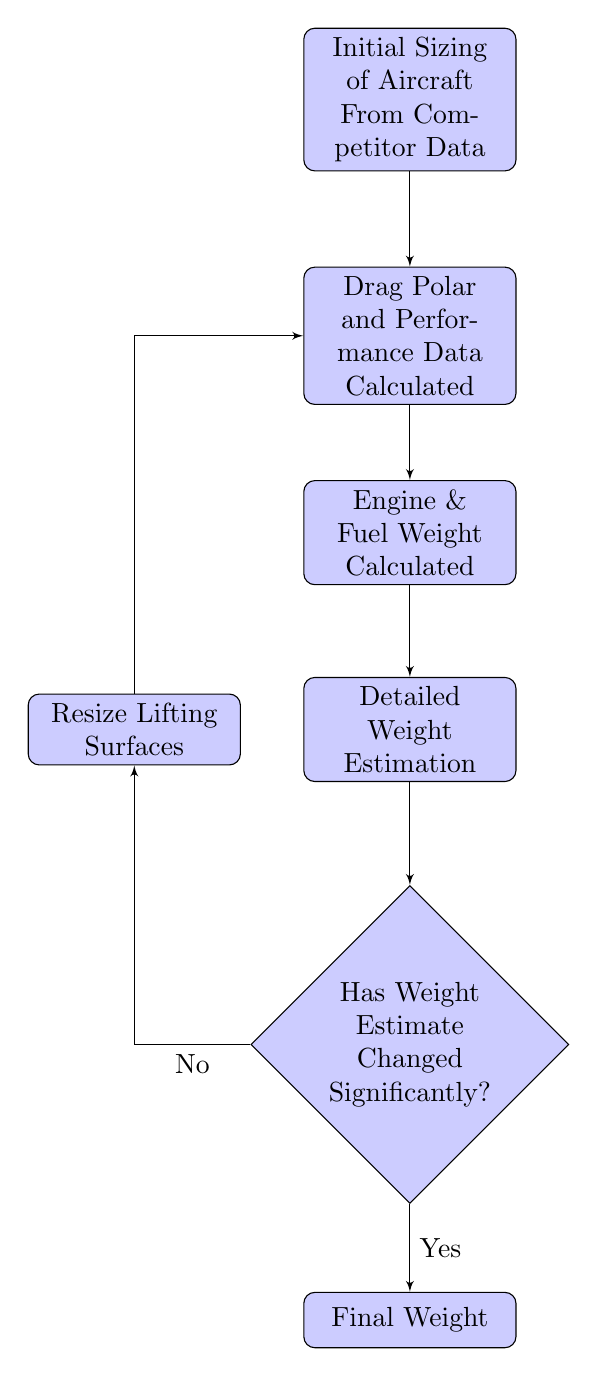
\begin{tikzpicture}[node distance = 2.2cm, auto]
    % Place nodes
    \node [block] (init) {Initial Sizing of Aircraft From Competitor Data};
    \node [block, below of=init, node distance = 3cm] (kit) {Drag Polar and Performance Data Calculated};
    \node [block, below of=kit, node distance = 2.5cm] (josh) {Engine \& Fuel Weight Calculated};
    \node [block, below of=josh, node distance = 2.5cm] (xavi) {Detailed Weight Estimation};
    \node [decision, below of=xavi, node distance = 4cm] (sig) {Has Weight Estimate Changed Significantly?};
    \node [block, below of=sig, node distance = 3.5cm] (stop) {Final Weight};
    \node [block, left of=xavi, node distance=3.5cm] (size) {Resize Lifting Surfaces};
    % Draw edges
    \path [line] (init) -- (kit);
    \path [line] (kit) -- (josh);
    \path [line] (josh) -- (xavi);
    \path [line] (xavi) -- (sig);
    \path [line] (sig) -| node [near start]{No}(size);
    \path [line] (size) |- (kit);
    \path [line] (sig) -- node{Yes}(stop);
\end{tikzpicture}
\end{center}
\caption{Information Flow For Weight Estimation}
\label{fig:flow}
\end{figure}


\begin{table}[!h]
\centering %HTP Table
\ra{1.3}
\begin{tabular}{@{}llll@{}}\toprule
$Component$ & $Technology$ & $Weight \ Saved \ (\%)$ & $Weight \ Saved \ (kg)$ \\
\midrule
Wing & Composites Skin Spars, Ribs & 15 & 607 \\
Fuselage & Composites Skin \& Stringers & 15 & 626 \\ 
Empennage & Composites Skin Spars, Ribs & 15 & 74  \\
Flight Controls & Fly-by-Wire & 15 & 27 \\ 
\midrule
\textbf{Total Saving} & & & 1,334 \\
\bottomrule
\end{tabular}
\caption{Weight Savings}
\label{table:wsave}
\end{table}

\begin{table}[p]
\centering
\ra{1}
\begin{tabular}{lrrr}\toprule

$Component$&$ Weight \ (kg)$&$x \ (m$)&$ z \ (m)$\\
 \midrule
\textbf{Structure}\\
Wing Group& 3,439  & 13.46 & 4.84 \\
Fuselage Group& 3,545 &13.89&2.70\\
Horizontal \ Tailplane&198& 25.17& 9.17\\
Vertical \ Tailplane& 229 & 23.79 &  6.13\\
Nose Gear & 131 & 3.23 & 1.4 \\
Main Gear&961&13.5&1.33\\
Engines & 4,020 & 11.33 & 4.40 \\
\textbf{Fixed Equipment}\\
Fuel Systems& 129 & 13.74 & 4.84\\
Flight Controls & 179 & 16.67 & 4.84\\
Hydraulics&314& 13.45 &3.8\\
Avionics&282&4.39&1.55\\
Electrical Systems&502&8.48&3.8\\
Air Cond. Systems&939&11.40&1.75\\
Furnishings&267& 13.3 &2.10\\
\textbf{Operators Items}\\
\underline{\textit{Fluids and Documenation:}}\\
Unusable Fuel& 14 & 13.46 &4.84\\
Oil For Engine IDG & 95 & 12.36 & 4.84 \\
Water for Galleys and Toilet&190& 26 & 3 \\
Toilet Rinse&60& 4.5 &4.17\\
Toilet System Pre-Charge& 36 & 4.5 & 4.17 \\
Aircraft Documents& 46 & 3.5 & 3.22 \\
\underline{\textit{Seating:}}\\
Passenger Seats & 1500 & 13.98 & 3\\
\underline{\textit{Galleys:}}\\
Galleys Structure & 100 & 23.4 & 3\\
Galley Fixed Equipment & 100 & 23.4 & 3\\
Catering & 300 & 23.4 & 3\\
\underline{\textit{Emergency Equipment:}}\\
Emergency Slides & 137 & 13.72 & 2.33\\
Aircraft Dependednt & 50 & 12.11 & 3 \\
Passenger Dependent & 30 & 13.98 & 2.8 \\
\underline{\textit{Crew:}}\\
Flight Crew & 190 & 3 & 3\\
Cabin Crew & 170 & 13.82 & 3\\
\textbf{Fuel and Payload}\\
Fuel & 3345 & 13.46 & 4.84\\
Passengers \& Carry On & 7659 & 13.98 & 2.70\\
Front Hold Baggage & 920 & 7.60 & 1.80\\
Rear Hold Baggage & 920 & 18.61 & 1.80\\

\bottomrule
\end{tabular}
\caption{Full Weight Breakdown of The A3U10}
\label{table:WXYZ}
\end{table}

\subsection{Design Weights}

The design weights were calculated using the weights in Table \ref{table:WXYZ} and the rules defined in the specification \cite{SPEC}. \\
The Basic MWE and Evaluation MWE are defined in equations \ref{eq:MWE} and \ref{eq:EMWE}. The values of Customer Changes and MWE Conservatism are 1\% and 2\% of Basic MWE respectively.

\begin{equation} \label{eq:MWE}
\centering
 Basic \ MWE = \sum{Structure \ Weights} + \sum{Fixed \ Equipment} + W_{furn}
\end{equation} 

\begin{equation} \label{eq:EMWE}
\centering
Evaluation \ MWE = Basic \ MWE + Customer \ Changes + MWE \ Conservatism
\end{equation}

The OWE weights, as defined by the specification, are given by equations \ref{eq:OWE} and \ref{eq:EOWE}, with OWE Conservatism taking the value of 1\% Basic OWE.

\begin{equation} \label{eq:OWE}
\centering
Basic \ OWE = Evaluation \ MWE + Operator Items 
\end{equation}


\begin{equation} \label{eq:EOWE}
\centering
Evaluation \ OWE = Basic \ OWE  + OWE \ Conservatism
\end{equation}

Using the Evaluation OWE and adding the SPP (standard passenger payload) gives the MZFW (maximum zero fuel weight) as shown in equation \ref{eq:mzfw}.

\begin{equation} \label{eq:mzfw}
\centering
MZFW = Evaluation \ OWE + SPP
\end{equation}

It is then possible to find the MRW (maximum ramp weight) by adding the mission block fuel and reserves, calculated by the propulsion specialist, to the MZFW as shown in equation \ref{eq:mrw}.

\begin{equation} \label{eq:mrw}
\centering
MRW = MZFW + Mission \ Block \ Fuel + Hold \ Fuel + Diversion \ Fuel
\end{equation}

The MTOW was found by subtracting the taxi-out fuel defined in the specification as 25kg from the MRW as shown in equation \ref{eq:mtow}.

\begin{equation} \label{eq:mtow}
\centering
MTOW = MRW - Tax-out \ Fuel
\end{equation}

The final design weight calculated was the MLW (maximum landing weight). As the A3UX family is designed for multiple short hops the MLW must be close to the MTOW than medium and long range aircraft. It is important that the aircraft is able land after a 300nm mission starting at MTOW. Therefore a third of the mission block fuel (for 3 x 300nm hops) was removed from the MTOW to give a MLW. The first hop will use more than one third of the mission block fuel as the aircraft is heaviest on this journey but this should allow for tail winds which would reduce fuel burn. The formula used for MLW is given by equation \ref{eq:mlw}.

\begin{equation} \label{eq:mlw}
\centering
MLW = MTOW - (Mission \ Block \ Fuel) / 3
\end{equation}

The parameters needed to calculate the design weights are displayed in Table \ref{table:dwp} and the design weights are shown in Table \ref{table:DW}.

\begin{table}[!h]
\centering %DESIGN WEIGHTS Table
\ra{1.3}
\begin{tabular}{@{}llll@{}}\toprule
$Paramater$ & $Weight \ (kg)$ \\
\midrule
Structures Total & 12,651  \\
Fixed Equipment Total & 2,217 \\ 
Furnishing Weight & 267 \\
Operators Items Total &3014\\
SPP& 9500 \\ 
Mission Block Fuel &2,653\\
Hold Fuel &338 \\
Reserve Fuel &354 \\
Taxi-out Fuel &25\\ 
\bottomrule
\end{tabular}
\caption{Parameters For Design Weight Calculations}
\label{table:dwp}
\end{table}

\begin{table}[!h]
\centering %HTP Table
\ra{1.3}
\begin{tabular}{@{}ll@{}}\toprule
$Paramater$ & $Weight \ (kg)$ \\
\midrule
Evaluation MWE & 15,590  \\
Evaluation OWE & 18,790 \\ 
MZFW & 28290 \\
MRW & 31,700\\
MTOW&   31,675 \\ 
MLW & 30,790 \\ 
\bottomrule
\end{tabular}
\caption{Parameters For Design Weight Calculations}
\label{table:DW}
\end{table}

\FloatBarrier

The design weights align with the prediction in the preliminary design stage base on similar aircraft. For example aircraft MTOW against number of passengers for turboprop aircraft in the regional category to find a predicted MTOW. The data is shown in Figure \ref{fig:mtowvpax} and a predicted MTOW of 30,500kg was read from the graph for a 100 seater regional turboprop. The A3U10 is slightly heavier than this at 31,675kg but still within the expected range. It was hoped that the aircraft would be lighter than predicted by competition aircraft data as a heavier aircraft generally has higher fuel burn, a direct contributor to DOC. Judging the aircraft on MTOW per passenger is slightly flawed however as it can be skewed by aircraft with small fuel capacities. It is better to judge the efficiency of the airframe on the operating weight empty per passenger. In this regard the A3U10 compares favorably to the main competitors: the ATR 72-600 and Bombardier Dash 8 Q400 as shown in Table \ref{table:OWEpp}. This can be attributed to the extensive use of composites; the Dash 8 performs poorly on this metric as it's primary structure is metallic. On the other hand the he ATR 72-600 structure is approximately 20\% composite \cite{atrcomp} and so has a much lower OWE/PAX ratio. The A3U10 is even better which can be attributed to the composite fuselage which the ATR 72-600 does not have. Without the 626kg saved by the composite fuselage the A3U10 would be 1kg/PAX heavier than the ATR 72-600 at 194kg/PAX. 

\FloatBarrier
\begin{figure} 
\centering
\includegraphics[width=0.9\textwidth]{mtow_pax.PNG}
\caption{MTOW Against Passenger Capacity}
\label{fig:mtowvpax}
\end{figure}
\FloatBarrier

\FloatBarrier
\begin{table}[!h]
\centering %HTP Table
\ra{1.3}
\begin{tabular}{@{}lrrr@{}}\toprule
 & $ATR 72-600$ & Dash 8 Q400 & A3U10\\
\midrule
Passenger Capacity & 70 & 80 & 100  \\
OWE (kg)  & 13,500 & 17,819 & 18,790 \\ 
OWE / PAX (kg) & 193 & 217 & 188 \\
\bottomrule
\end{tabular}
\caption{Comparison of Airframe Efficiency}
\label{table:OWEpp}
\end{table}
\FloatBarrier

\subsection{Moments Of Inertia}

Moment of inertia calculation were required for stability and control calculation. As the technical integrator had authority over weights and layout the role was most appropriate for these calculations. To simplify the calculations the each of the weight components in Table \ref{table:WXYZ} were modelled as point masses at the $x$ and $z$ locations stated in the table and inertias were only calculated at MTOW. Firstly the centre of gravity in the $x$ direction, $x_{cg}$, and $z$ direction, $z_{cg}$ were found using equations \ref{eq:xcg} and \ref{eq:zcg} respectively. It is worth noting $\sum w_{i}\neq MTOW$ as conservatism factors have been ignored for these calculations. The results of the calculation are shown in Table \ref{table:inert}.


\begin{equation} \label{eq:xcg}
\centering
x_{cg} = \frac{ \sum_{i}^{n}(W_{i}*x_{i})}{ \sum_{i}^{n} W_{i}}
\end{equation}

\begin{equation} \label{eq:zcg}
\centering
z_{cg} = \frac{ \sum_{i}^{n}(W_{i}*z_{i})}{ \sum_{i}^{n} W_{i}}
\end{equation}


\begin{equation} \label{eq:zcg}
\centering
z_{cg} = \frac{ \sum_{i}^{n}(W_{i}*z_{i})}{ \sum_{i}^{n} W_{i}}
\end{equation}

\begin{equation} \label{eq:iyy}
\centering
I_{yy} =  \sum_{i}^{n}w_{i}*\Big[(z_{i}-z_{cg})^2 + (z_{i}-z_{cg})^2 \Big]
\end{equation}

\begin{equation} \label{eq:izx}
\centering
I_{zx} =  \sum_{i}^{n}w_{i}*\Big[(z_{i}-z_{cg})*(z_{i}-z_{cg})\Big]
\end{equation}

\begin{table}[!h]
\centering %HTP Table
\ra{1.3}
\begin{tabular}{@{}ll@{}}\toprule
$x_{cg}$ & = 13.39m \\
$z_{cg}$  &= 3.40m  \\ 
$I_{yy}$ &= 63,900kgm$^2$ \\
$I_{zx}$ &= 3,290kgm$^2$\\
\bottomrule
\end{tabular}
\caption{CG Locations and Inertias at MTOW}
\label{table:inert}
\end{table}
\FloatBarrier

\section{Balance Diagram}

\section{DOC Case Study For Composite Use}

The target DOC reduction outlined by the specification was 15\%. Therefore the use of carbon fibre reinforced polymer and other composites for the wing, empennage and fuselage must be justified on terms of achieving this target. As the composite fuselage would be a market first for regional truboprops it would have been best to evaluate it's DOC impact directly. This was not practical however as there was not enough accurate data specifically on fuselage costs to evaluate the change in aircraft price soley due to that design feature. Therefore the use of composites compared to an all alluminium frame, with composite nacelles and propellors, was analysed instead. This is similar to the Bombardier Dash 8 Q400 airframe so the analysis is crude comparison with this competitor. \\
The unit cost of the aircraft was calculated using the Roskam method \cite{R8}. The result was a 33\% increase in the cost per unit for the composite aircraft, with a 25\% added to unit cost to give the first price for the aircraft. The cost of interest repayments was expected to be approximately and additional 10\% so the profit margin will be approximately 15\% for both aircraft. The aircraft MTOW is reduced 6.8\% for the composite aircraft, with fuel and engine weight, as calculated by the propulsion expert, both significantly higher for the alluminium aircraft.



\pagebreak


\pagebreak



\pagebreak

\begin{thebibliography}{9}
%Last name, First Initial, Year published. Title. Publisher, Volume, Page(s).
% HARVARD REFERENCE STYLE:
%Brunner, F.H., 1949. Synthetic gasoline from natural gas. Industrial and engineering chemistry, 41(11), pp.2511-2515.
\bibitem{CS25} 
European Aviation Safety Agency (EASA), 2007.
\textit{Certification Specifications for Large Aeroplanes: CS-25. Amendment 3.}

\bibitem{GAPP} 
Macgregor, K., 2017.
\textit{General Arrangement Drawings: An Introduction To Aircraft Geometry}
Airbus Group.

\bibitem{SUGAR}
Bradley, M K. and Droney, C.K.  , 2012.
\textit{Subsonic Ultra Green Aircraft Research Phase II: N+4 Advanced Concept Development}
Boeing Research and Technology
 

\bibitem{R2}
Roskam, J., 1985. 
\textit{Airplane Design, Part II : Preliminary Configuration Design and Integration of the Propulsion System.}
The University of Kansas.

\bibitem{SCHMITT}
SCHMITT, 2017.
\textit{6. Fuselage Design}
University of Hamberg

\bibitem{R3}
Roskam, J., 1985.
\textit{Airplane Design Part III: Layout Design of Cockpit, Fuselage, Wing and Empennage: Cutaways and Inboard Profiles.}
The University of Kansas.

\bibitem{tbeek}
 Torenbeek, E. 1982.
\textit{Synthesis of Subsonic Airplane Design}
Kluwer Academic Publishers. 

\bibitem{kit}
Thornton, K., 2018.
\textit{Phase 3 Primary Report:Aerodynamics.}
University of Bath: CTA1 – Aerospace Group Business \& Design Project II.

\bibitem{jenk}
Jenkinson. L.R., 1999.
\textit{Civil Jet Aircraft Design.}
Butterworth-Heinemann.

\bibitem{josh}
Bowen, J. 2018.
\textit{Phase 3 Primary Report: Propulsion.}
University of Bath: CTA1 – Aerospace Group Business \& Design Project II.

\bibitem{R5}
Roskam, J., 1985.
\textit{Airplane Design Part V: Component Weight Estimation}
The University of Kansas.

\bibitem{R8}
Roskam, J., 1985.
\textit{Airplane Design Part VIII: Airplane Cost Estimation: Design, Development, Manufacturing and Operating.}
The University of Kansas.

\bibitem{guide}
A. Nag, S.S. Patel, S.A. Akbar, 2013.
\textit{Fuzzy Logic Based Depth Control of an Autonomous Underwater Vehicle.}
Unknown Publisher. 

\bibitem{jane}
P. Jackson et al, 2013.
\textit{JANE'S ALL THE WORLD'S AIRCRAFT}
IHS. 

\bibitem{atr_guide}
A. Nag, S.S. Patel, S.A. Akbar, 2013.
\textit{Fuzzy Logic Based Depth Control of an Autonomous Underwater Vehicle.}
Unknown Publisher. 

\bibitem{bae146}
European Aviation Safety Agency (EASA), 2015.
\textit{Type Certificate Data Sheet: BAe 146 / AVRO 146-RJ Series}

\bibitem{q400}
Bombardier Inc., 2014.
\textit{Bombardier Dash 8 Series 400 Airport Planning Manual}
Bombardier Inc..

\bibitem{atrcomp}
ATR Website: http://www.atraircraft.com/about-atr/corporate-overview/company-profile.html

\bibitem{tony}
Tony Hewitt., April 2018.
\textit{Technical Surgery, University of Bath}


\end{thebibliography}

\pagebreak
\section*{Appendices}
\subsection*{Appendix A}
\newpage
\subsection{Appendix B}
%\begin{figure}[h!]
%\centering
%\includegraphics[width=0.9\textwidth]{henbury}
%\caption{Email confirmation of pool rental at Henbury Leisure Center}
%\label{fig:henbury}
%\end{figure}
\end{document}

%%%Run this in cmd
%	pdflatex BasicFile.tex 
%	pdflatex BasicFile.tex 
%	makeindex -s TI_Report.ist -t TI_Report.slg -o TI_Report.syi TI_Report.syg
%	makeindex -s BasicFile.ist -t BasicFile.glg -o BasicFile.gls Report_Base_v6.glo 
%	pdflatex BasicFile.tex
%	BasicFile.pdf